\Aufgabe[e]{Trigonometrische Gleichungen}{
Bestimmen Sie die L\"osungsmenge der folgenden Ausdr\"ucke.
Beachten Sie dabei die Periodizit\"at der Funktionen.
Skizzieren Sie die Funktionen, um Ihre Ergebnisse zu best\"atigen.

\begin{abc}
\item $\sin^2(x) = \displaystyle\frac{1}{2}$\,.

\item $\sin^2(x) - \cos^2(x) + \sin(x) = 0$\,.

\item $\cot^2(x)+\cot(x) = 0$ \quad with \quad
$\cot(x) = \displaystyle \frac{1}{\tan(x)}
= \displaystyle \frac{\cos(x)}{\sin(x)}$\,.

\item $\sin(x) \cos(x) = \displaystyle\frac{1}{2}$\,.

\item $\displaystyle\frac{\tan(x)+1}{\tan(x)-1} = 2 + \sqrt{3}$\,.
\end{abc}
}

\Loesung{

\textbf{a)} Die L\"osungsmenge von $\sin^2(x) = \displaystyle\frac{1}{2}$ ist 
$$
x \in \left\{
\frac{\pi}{4} + \frac{\pi}{2} k\,,\quad
k \in \mathbb{Z}
\right\}\,.
$$

\begin{minipage}{\linewidth}
\centering

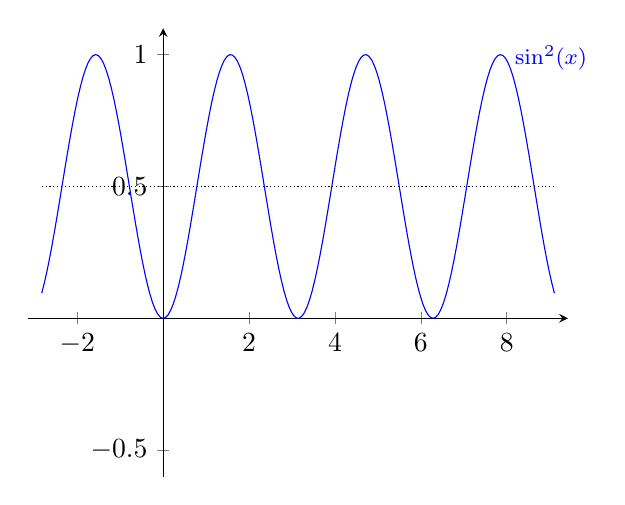
\begin{tikzpicture}
\begin{axis}[
axis lines=middle,
clip=false,
xmin=-pi,
xmax=3*pi,
ymin=-.6,
ymax=1.1,
%xlabel=$x$,
%ylabel=$y$,
xticklabel style={black}
]

\addplot[domain=-.9*pi:2.9*pi,samples=200,blue]{sin(deg(x))^2}
node[right,pos=0.9,font=\footnotesize]{$\sin^2(x)$};

\addplot[domain=-.9*pi:2.9*pi,black,densely dotted]{0.5};

\end{axis}
\end{tikzpicture}

\end{minipage}


\newpage
%\bigskip
\textbf{b)} Um die L\"osungsmenge von $f(x) = 0$ mit
$f(x) := \sin^2(x) - \cos^2(x) + \sin(x)$ zu bestimmen, nutzen die Pythagoreische Identit\"at f\"ur
trigonometrische Funktionen,
$$
\text{\fbox{$\cos^2(x) + \sin^2(x) = 1$}}\,.
$$

Ausnutzen von $\cos^2(x) = 1 - \sin^2(x)$ f\"uhrt zu
$$
\begin{array}{rcl}
f(x) &=& 0\,,\\[1ex]
\sin^2(x) - \cos^2(x) + \sin(x) &=& 0\,,\\[1ex]
\sin^2(x) - (1 - \sin^2(x)) + \sin(x) &=& 0\,,\\[1ex]
2 \cdot \sin^2(x) + \sin(x) -1 &=& 0\,.
\end{array}
$$

Wir substituieren $y:=\sin(x)$ und erhalten die quadratische Gleichung
$$
2y^2 + y -1 = 0\,,
$$
mit den L\"osungen $y_1=-1$ und $y_2=\frac{1}{2}$.
Das f\"uhrt zu den folgenden Gleichungen 
$$
\sin(x) = -1\quad \text{ and }\quad
\sin(x) = \frac{1}{2}\,.
$$

Die L\"osungsmenge von $\sin^2(x) - \cos^2(x) + \sin(x) = 0$ ist
$$
x \in \left\{
\frac{\pi}{6} + 2 \pi k\,,\quad
\frac{5 \pi}{6} + 2 \pi k\,,\quad
\frac{9 \pi}{6} + 2 \pi k\,,\quad
k \in \mathbb{Z}
\right\}\,.
$$

\begin{minipage}{\linewidth}
\centering

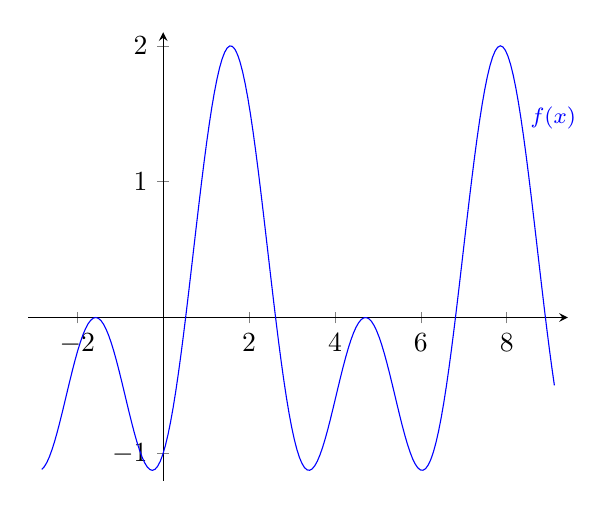
\begin{tikzpicture}
\begin{axis}[
axis lines=middle,
clip=false,
xmin=-1*pi,
xmax=3*pi,
ymin=-1.2,
ymax=2.1,
%xlabel=$x$,
%ylabel=$y$,
xticklabel style={black}
]

\addplot[domain=-.9*pi:2.9*pi,samples=200,blue]{%
sin(deg(x))^2-cos(deg(x))^2+sin(deg(x))}
node[right,pos=0.9,font=\footnotesize]{$f(x)$};

\end{axis}
\end{tikzpicture}

\end{minipage}

\newpage
%\bigskip
\textbf{c)} Der Kotangens ist definiert als
$$
\text{\fbox{$\cot(x) = \displaystyle \frac{1}{\tan(x)}
= \displaystyle \frac{\cos(x)}{\sin(x)}$}}\,.
$$

\begin{minipage}{\linewidth}
\centering

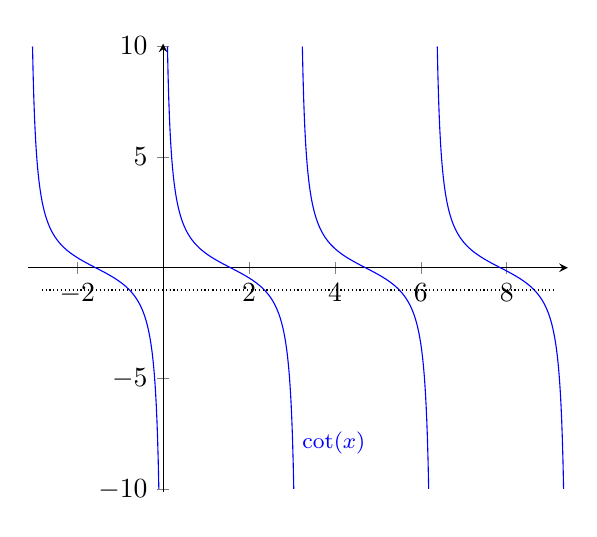
\begin{tikzpicture}
\begin{axis}[
axis lines=middle,
clip=false,
xmin=-1*pi,
xmax=3*pi,
ymin=-10.1,
ymax=10.1,
%xlabel=$x$,
%ylabel=$y$,
xticklabel style={black}
]

\addplot[domain=0+.1-pi:pi-.1-pi,samples=200,blue]{cot( deg(x) )};

\addplot[domain=0+.1:pi-.1,samples=200,blue]{cot( deg(x) )}
node[right,pos=0.9,font=\footnotesize]{$\cot(x)$};

\addplot[domain=0+.1+pi:pi-.1+pi,samples=200,blue]{cot( deg(x) )};

\addplot[domain=0+.1+2*pi:pi-.1+2*pi,samples=200,blue]{cot( deg(x) )};

\addplot[domain=-.9*pi:2.9*pi,black,densely dotted]{-1.0};

\end{axis}
\end{tikzpicture}

\end{minipage}

\bigskip
Die Gleichung $\cot^2(x)+\cot(x) = 0$ kann geschrieben werden als
$$
\cot(x) \cdot \left(\cot(x)+1\right) = 0\,,
$$
die Gleichung ist erf\"ullt, wenn
$$
\cot(x) = 0\quad \text{ und }\quad
\cot(x) = -1\,.
$$

\medskip
Aus diesen beiden Bedingungen ergibt sich die L\"osungsmenge von
$f(x) := \cot^2(x)+\cot(x) = 0$ als
$$
x \in \left\{
\frac{\pi}{2} + \pi k\,,\quad
\frac{3 \pi}{4} + \pi k\,,\quad
k \in \mathbb{Z}
\right\}\,.
$$

\begin{minipage}{\linewidth}
\centering

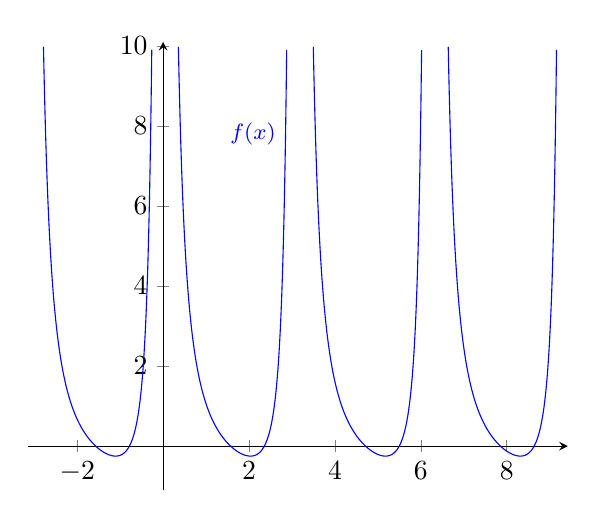
\begin{tikzpicture}
\begin{axis}[
axis lines=middle,
clip=false,
xmin=-1*pi,
xmax=3*pi,
ymin=-1.1,
ymax=10.1,
%xlabel=$x$,
%ylabel=$y$,
xticklabel style={black}
]

\addplot[domain=0+.355-pi:pi-.265-pi,samples=200,blue]{%
cot(deg(x))*(cot(deg(x)) + 1)};

\addplot[domain=0+.355:pi-.265,samples=200,blue]{%
cot(deg(x))*(cot(deg(x)) + 1)}
node[left,pos=0.9,font=\footnotesize]{$f(x)$};

\addplot[domain=0+.355+pi:pi-.265+pi,samples=200,blue]{%
cot(deg(x))*(cot(deg(x)) + 1)};

\addplot[domain=0+.355+2*pi:pi-.265+2*pi,samples=200,blue]{%
cot(deg(x))*(cot(deg(x)) + 1)};

\end{axis}
\end{tikzpicture}

\end{minipage}


\newpage
%\bigskip
\textbf{d)} Betrachten Sie das Additionstheorem f\"ur trigonometrische Funktionen
$$
\text{\fbox{$ \sin(\varphi+\psi) = \sin(\varphi) \cos(\psi) +
\cos(\varphi) \sin(\psi)
$}}\,.
$$

Um die L\"osungsmenge von $\sin(x) \cos(x) = \frac{1}{2}$,
zu bestimmen, nutzen wir
$$
\sin(x) \cos(x) = \frac{1}{2} \cdot \sin(2x)
$$
mit dem Additionstheorem.
Die urspr\"ungliche Gleichung kann geschrieben werden als
$$
\sin(2x) = 1.
$$

Die Substitution $y:=2x$ f\"uhrt zu $\sin(y) = 1$ mit der L\"osung
$$
y \in \left\{
\frac{\pi}{2} + 2\pi k\,,\quad
k\in \mathbb{Z}
\right\}\,.
$$

Die L\"osungsmenge von $f(x) = \frac{1}{2}$,
$f(x) := \sin(x) \cos(x)$ ist
$$
x \in \left\{
\frac{\pi}{4} + \pi k\,,\quad
k\in \mathbb{Z}
\right\}\,.
$$


\begin{minipage}{\linewidth}
\centering

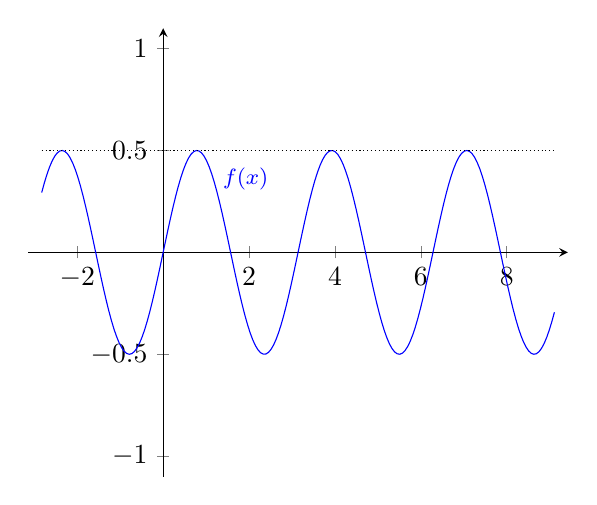
\begin{tikzpicture}
\begin{axis}[
axis lines=middle,
clip=false,
xmin=-pi,
xmax=3*pi,
ymin=-1.1,
ymax=1.1,
%xlabel=$x$,
%ylabel=$y$,
xticklabel style={black}
]

\addplot[domain=-.9*pi:2.9*pi,samples=200,blue]{sin(deg(x))*cos(deg(x))}
node[right,pos=0.33,font=\footnotesize]{$f(x)$};

\addplot[domain=-.9*pi:2.9*pi,black,densely dotted]{0.5};

\end{axis}
\end{tikzpicture}

\end{minipage}


\newpage
\bigskip
\textbf{e)} Wir schreiben die Gleichung um zu
$$
\begin{array}{rcl}
\displaystyle\frac{\tan(x)+1}{\tan(x)-1} &=& 2 + \sqrt{3}\,,\\[3ex]
\displaystyle\frac{\tan(x)+1+(1-1)}{\tan(x)-1} &=& 2 + \sqrt{3}\,,\\[3ex]
\displaystyle\frac{(\tan(x)-1)+2}{(\tan(x)-1)} &=& 2 + \sqrt{3}\,,\\[3ex]
1 + \displaystyle\frac{2}{\tan(x)-1} &=& 2 + \sqrt{3}\,.
\end{array}
$$

Aufl\"osen der Gleichung nach $\tan(x)$ f\"uhrt zu ( f\"ur $\tan(x) \neq 1$)
$$
\tan(x)
= \frac{2}{1+\sqrt{3}}+1
= \frac{3+\sqrt{3}}{1+\sqrt{3}}=\sqrt{3}\,.
$$

Die L\"osungsmenge von 
$$
\displaystyle\frac{\tan(x)+1}{\tan(x)-1} = 2 + \sqrt{3}
$$
ist \"aquivalent zu der L\"osungsmenge von $\tan(x)=\sqrt{3}$ und
ist daher gegeben durch
$$
x \in \left\{
\frac{\pi}{3} + \pi k\,,\quad
k\in \mathbb{Z}
\right\}\,.
$$

\begin{minipage}{\linewidth}
\centering

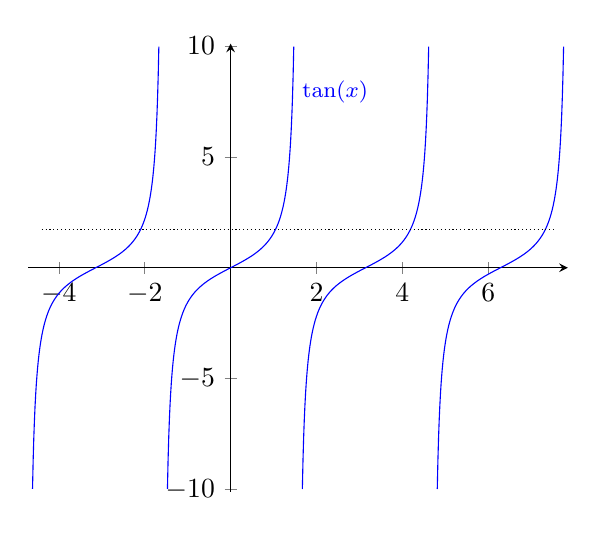
\begin{tikzpicture}
\begin{axis}[
axis lines=middle,
clip=false,
xmin=-1.5*pi,
xmax=2.5*pi,
ymin=-10.1,
ymax=10.1,
%xlabel=$x$,
%ylabel=$y$,
xticklabel style={black}
]

\addplot[domain=-pi/2+.1-pi:pi/2-.1-pi,samples=200,blue]{tan( deg(x) )};

\addplot[domain=-pi/2+.1:pi/2-.1,samples=200,blue]{tan( deg(x) )}
node[right,pos=0.9,font=\footnotesize]{$\tan(x)$};

\addplot[domain=-pi/2+.1+pi:pi/2-.1+pi,samples=200,blue]{tan( deg(x) )};

\addplot[domain=-pi/2+.1+2*pi:pi/2-.1+2*pi,samples=200,blue]{tan( deg(x) )};

\addplot[domain=-1.4*pi:2.4*pi,black,densely dotted]{sqrt(3)};

\end{axis}
\end{tikzpicture}

\end{minipage}

}
